\section{Application to ACLED 2018--2024}\label{sec:application}

All models are trained on 2018--2022 and evaluated on 2023--2024. The boosting models
use the features and hyperparameters of \citet{menicali2026conflicts}. The computations
were run on the Notre Dame Center for Research Computing.

\subsection{Reconstructing the cell-week table}\label{sec:app-data}

The table built by the original pipeline has 70{,}033{,}444 rows but only 34{,}671{,}180
distinct cell-weeks, so 50.5\% of its rows are copies. One partition shows the pattern:
613{,}459 cell-weeks appear once, while others appear 2, 3, 8, 16, 32, 48 and up to 648
times. These multiplicities are products of small integers. The national indicators and
IPC regions are attached by spatial intersection and then merged on cell and year, so a
cell that touches several countries is multiplied at every join, and each copy combines
indicators from different countries. We rebuilt the table with one row per cell-week, as
described in Section~\ref{sec:data-acled}. Excluding rock-and-ice cells leaves 59{,}344
cells and 366 weeks, or 21{,}719{,}904 cell-weeks. Of these, 4{,}787{,}224 fall in the
test period, in 46{,}031 cells with complete climate records. The prevalence of event
weeks in the test period is 1.62\% for conflict and 2.73\% for unrest. In the duplicated
table it is 2.98\% and 3.58\%, because the copied border cells have more events than
average.

\subsection{The boosting analysis before and after the repair}\label{sec:app-xgb}

Table~\ref{tab:app-xgb} reproduces the XGBoost analysis on the duplicated table, then
repeats it on the repaired table. In the corrected version the number of trees is chosen
on 2022 rather than on the test years. On the duplicated table we recover the published
performance: AUC-PR is 0.934 for conflict and 0.917 for unrest, against 0.93 and 0.91
reported. Split by cell type, however, nearly all of it comes from the duplicated border
cells, with AUC-PR 0.97. On interior cells AUC-PR is 0.50--0.53.

The reason is a feature-construction artefact. The four-week event counts are computed
row by row within each cell. When a cell-week has copies, the rows just before a given
row are copies of the same week, so for duplicated cells the ``past'' counts contain the
current week's events, which is the outcome. On the repaired table AUC-PR falls to 0.549
for conflict and 0.553 for unrest, with no difference between border and interior cells.
A persistence baseline that ranks cell-weeks by their past four-week event count reaches
0.511 and 0.500. The covariates therefore add about 0.04--0.05 AUC-PR to recent event
history. They are not the dominant source of skill implied by the published ranking.

\begin{table}
\caption{XGBoost on the 2023--2024 test period, as published (duplicated table, early
stopping on the test years) and corrected (one row per cell-week, early stopping on
2022). AUC-PR is also reported separately for cells that were duplicated in the
original table (``border'') and for the others (``interior'').}\label{tab:app-xgb}
\centering\small
% Generated by paper/make_real_figures.py; do not edit by hand.
% Inputs (sha256 prefix):
%   results_real/xgb/metrics_corrected_Conflict.json  8fb209c4452d
%   results_real/xgb/metrics_corrected_Unrest.json  17d551c67437
%   results_real/xgb/metrics_corrected_te_Conflict.json  4342ad67c6f3
%   results_real/xgb/metrics_corrected_te_Unrest.json  c27a32300605
%   results_real/xgb/metrics_dedup_Conflict.json  046b10c52ba8
%   results_real/xgb/metrics_dedup_Unrest.json  5370f7674a41
%   results_real/xgb/metrics_original_Conflict.json  37a6e6e5b933
%   results_real/xgb/metrics_original_Unrest.json  9c4718f1c2d2
\begin{tabular}{@{}llrrrcccc@{}}
\toprule
Pipeline & Outcome & Test rows & Prevalence & Trees & AUC-PR & \multicolumn{2}{c}{AUC-PR by cell} & Persistence \\
\cmidrule(lr){7-8}
 & & & & & & dup.\ in original & other cells & AUC-PR \\
\midrule
As published & Conflict & 14.43M & 2.98\% & 1998 & 0.934 & 0.966 & 0.498 & 0.882 \\
As published & Unrest & 14.43M & 3.58\% & 1474 & 0.917 & 0.968 & 0.528 & 0.843 \\
\addlinespace
Original procedure, repaired table & Conflict & 4.79M & 1.62\% & 488 & 0.546 & 0.590 & 0.523 & 0.481 \\
Original procedure, repaired table & Unrest & 4.79M & 2.73\% & 646 & 0.555 & 0.543 & 0.558 & 0.468 \\
\addlinespace
Corrected & Conflict & 4.79M & 1.62\% & 637 & 0.544 & 0.588 & 0.521 & 0.481 \\
Corrected & Unrest & 4.79M & 2.73\% & 814 & 0.557 & 0.545 & 0.559 & 0.468 \\
\addlinespace
Corrected + cell event rate & Conflict & 4.79M & 1.62\% & 381 & 0.566 & 0.598 & 0.549 & 0.481 \\
Corrected + cell event rate & Unrest & 4.79M & 2.73\% & 135 & 0.583 & 0.567 & 0.586 & 0.468 \\
\bottomrule
\end{tabular}

\end{table}

\subsection{Residual spatial structure and the hybrid model}\label{sec:app-hybrid}

We fit the hybrid model~\eqref{eq:hybrid} to Africa and the Middle East (longitude
$20^\circ$W to $65^\circ$E, latitude $36^\circ$S to $45^\circ$N; 13{,}719 cells). It
combines a spatially cross-fitted XGBoost offset, country effects and a Mat\'ern field
with sea cells as barriers (Remark~\ref{rem:boundary}). The offset's residuals have
strong spatial structure for conflict (Table~\ref{tab:app-field}): Moran's $I$ of the
cell residuals is 0.45 ($p = 0.005$), and the semivariogram rises over the first
$300$--$400$\,km before levelling off (Figure~\ref{fig:app-variogram}). Neighbouring
cells in the same country have more strongly correlated residuals (0.48) than
neighbours across a border (0.31), which points to country-level effects in addition to
the smooth field. Unrest residuals are much less structured: Moran's $I$ is 0.11, and
the within-country and across-border correlations are equal.

The estimated fields (Figure~\ref{fig:app-field}) are consistent with this. For
conflict, the field has a range of 277\,km and a standard deviation of 1.24 on the logit
scale. Its positive values form contiguous regions. Averaging $\hat w$ over boxes, the
highest values are in eastern Democratic Republic of the Congo (1.85), northern
Mozambique (1.65), Syria and Iraq (1.55), Yemen (1.36), the Lake Chad basin (1.35) and
the central Sahel (0.76); the Horn of Africa is weaker (0.33). In these regions conflict
is more frequent than the covariates and recent history predict. The clearest negative
regions are the Arabian interior ($-0.73$) and the western Congo basin ($-0.84$). The
unrest field has a range of only 72\,km and consists mainly of isolated cells rather
than regional patterns.

Adding the latent effects improves out-of-sample prediction for both outcomes
(Table~\ref{tab:app-hybrid}). For conflict, the log score falls from 0.0630 to 0.0600,
AUC-PR rises from 0.508 to 0.527 and AUC-ROC from 0.942 to 0.958. For unrest, the
corresponding figures are 0.0672 to 0.0633, 0.522 to 0.548 and 0.946 to 0.959.
\todo{Add the like-for-like comparison with the corrected XGBoost model on the same
Africa and Middle East test rows, with the cell-clustered standard error of the log-score
difference (CRC Task 6). The global fit (Task 7) follows.}

\begin{table}
\caption{Residual diagnostics of the spatially cross-fitted XGBoost model and
hyperparameters of the hybrid model, Africa and the Middle East.}\label{tab:app-field}
\centering\small
\begin{tabular}{@{}lcccccc@{}}
\toprule
Outcome & Moran's $I$ & \multicolumn{2}{c}{Neighbour residual corr.} & $\hat\rho_w$ (km) & $\hat\sigma_w$ & $\hat\sigma_u$ \\
 & & within country & across border & & & \\
\midrule
Conflict & 0.452 & 0.482 & 0.305 & 277 & 1.24 & 0.35 \\
Unrest & 0.110 & 0.114 & 0.108 & 72 & 1.11 & 0.59 \\
\bottomrule
\end{tabular}

\end{table}

\begin{table}
\caption{Out-of-sample scores, Africa and the Middle East, 2023--2024. Lower is better
for the log and Brier scores.}\label{tab:app-hybrid}
\centering\small
% Generated by paper/make_real_figures.py; do not edit by hand.
% Inputs (sha256 prefix):
%   results_real/compare/compare_conflict.json  f9cfaa08c2c7
%   results_real/compare/compare_unrest.json  b8e39ca9067c
\begin{tabular}{@{}llcccccc@{}}
\toprule
Outcome & Model & Log score & Brier & AUC-PR & AUC-ROC & \multicolumn{2}{c}{$\Delta$ log score $\times 10^3$ (SE)} \\
\cmidrule(lr){7-8}
 & & & & & & by cell & by country \\
\midrule
Conflict & XGBoost, corrected & 0.0618 & 0.0160 & 0.515 & 0.949 & \multicolumn{2}{c}{reference} \\
Conflict & XGBoost + cell event rate & 0.0583 & 0.0157 & 0.533 & 0.960 & -3.50 (0.23) & (1.27) \\
Conflict & XGBoost, cross-fitted by country & 0.0700 & 0.0174 & 0.461 & 0.923 & 8.24 (0.42) & (2.27) \\
Conflict & Cross-fitted XGBoost + $u$ + iid cell effects & 0.0609 & 0.0164 & 0.519 & 0.959 & -0.93 (0.20) & (0.89) \\
Conflict & Cross-fitted XGBoost + $u + w$ & 0.0606 & 0.0164 & 0.519 & 0.959 & -1.17 (0.21) & (0.94) \\
Conflict & xgb\_dedup & 0.0612 & 0.0159 & 0.518 & 0.950 & -0.61 (0.08) & (0.53) \\
Conflict & Persistence (past 4 weeks) & -- & -- & 0.446 & -- & -- & -- \\
\addlinespace
Unrest & XGBoost, corrected & 0.0660 & 0.0173 & 0.532 & 0.950 & \multicolumn{2}{c}{reference} \\
Unrest & XGBoost + cell event rate & 0.0628 & 0.0169 & 0.550 & 0.959 & -3.22 (0.20) & (0.78) \\
Unrest & XGBoost, cross-fitted by country & 0.0707 & 0.0182 & 0.493 & 0.938 & 4.74 (0.25) & (1.20) \\
Unrest & Cross-fitted XGBoost + $u$ + iid cell effects & 0.0640 & 0.0172 & 0.540 & 0.958 & -2.04 (0.17) & (0.67) \\
Unrest & Cross-fitted XGBoost + $u + w$ & 0.0639 & 0.0172 & 0.540 & 0.958 & -2.07 (0.17) & (0.66) \\
Unrest & xgb\_dedup & 0.0660 & 0.0173 & 0.534 & 0.950 & 0.00 (0.06) & (0.15) \\
Unrest & Persistence (past 4 weeks) & -- & -- & 0.451 & -- & -- & -- \\
\bottomrule
\end{tabular}

\end{table}

\begin{figure}
\centering
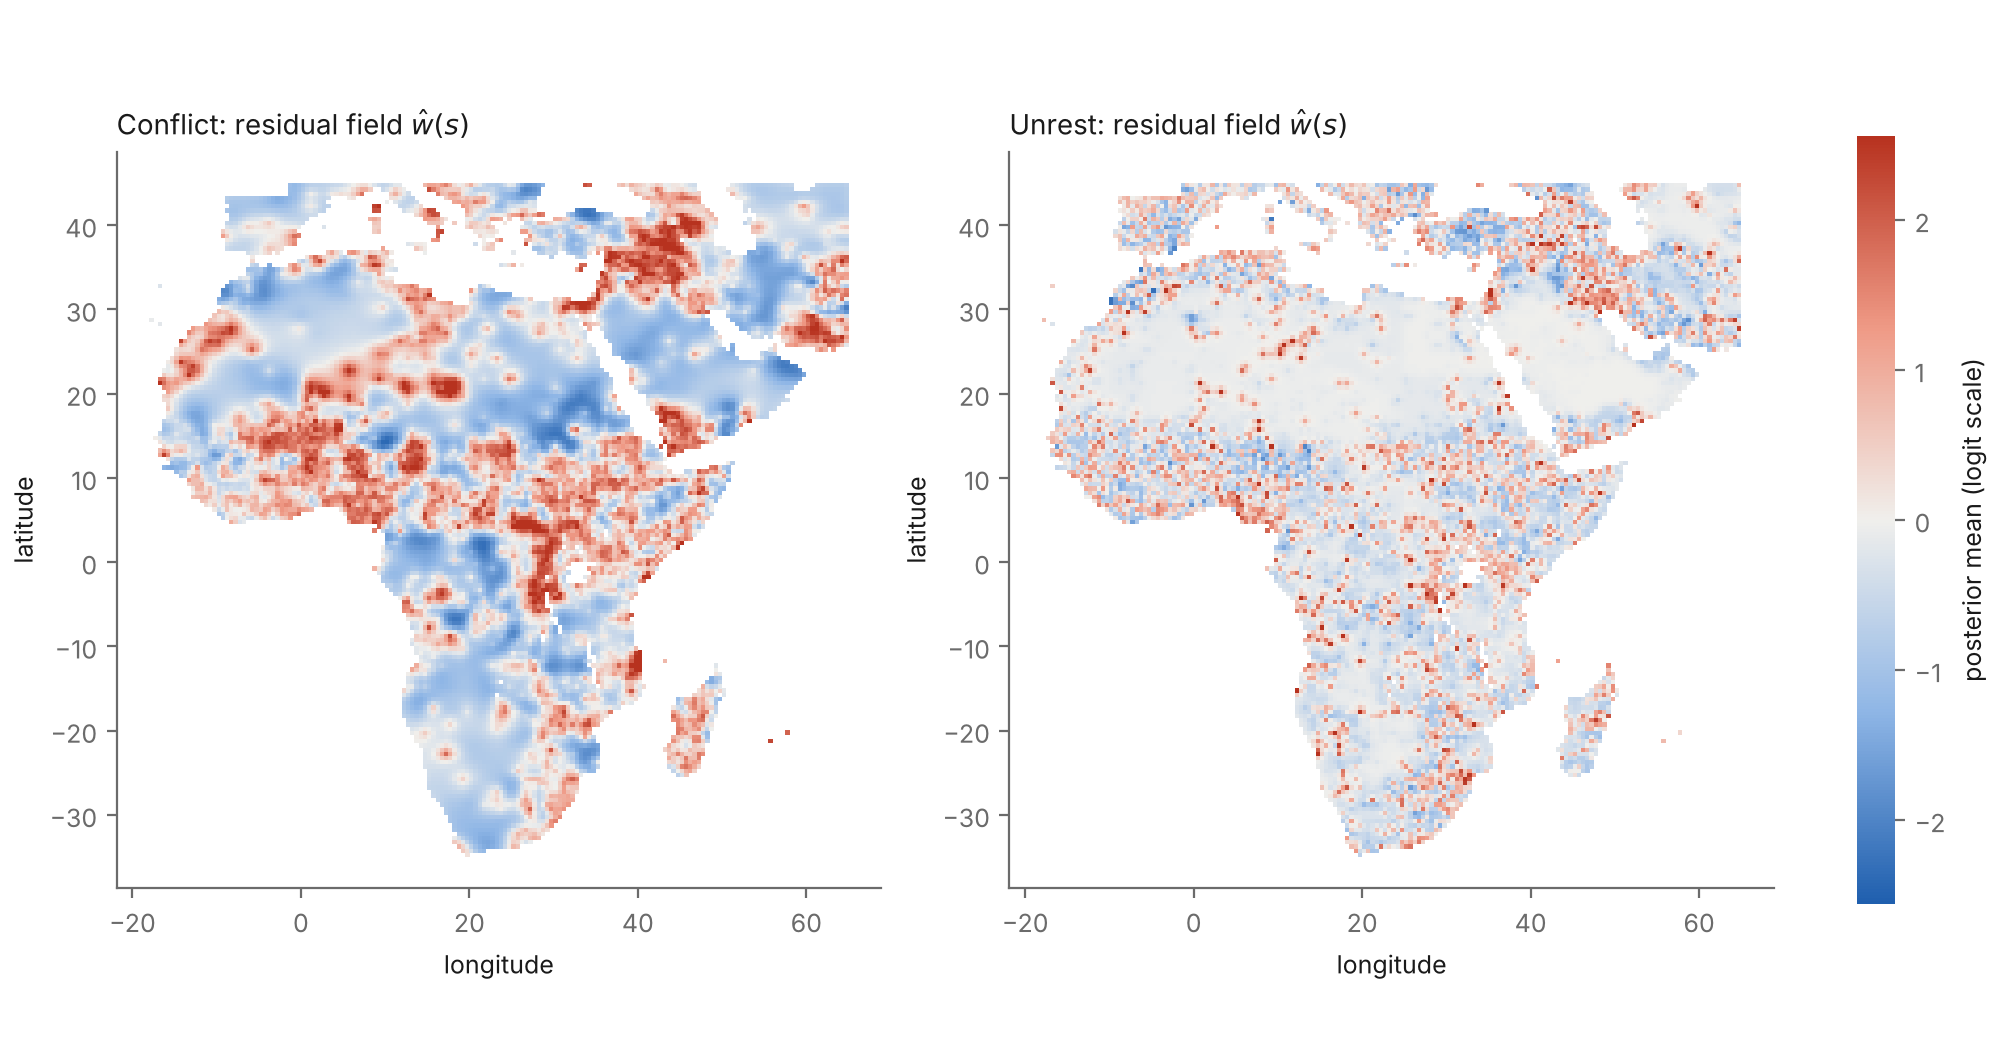
\includegraphics[width=\textwidth]{figures/real_field.png}
\caption{Posterior mean of the residual field $w(s)$ of the hybrid model for conflict
(left) and unrest (right), on the logit scale. Positive values mark persistently higher
risk than predicted by the covariates, recent event history and country
effects.}\label{fig:app-field}
\end{figure}

\begin{figure}
\centering
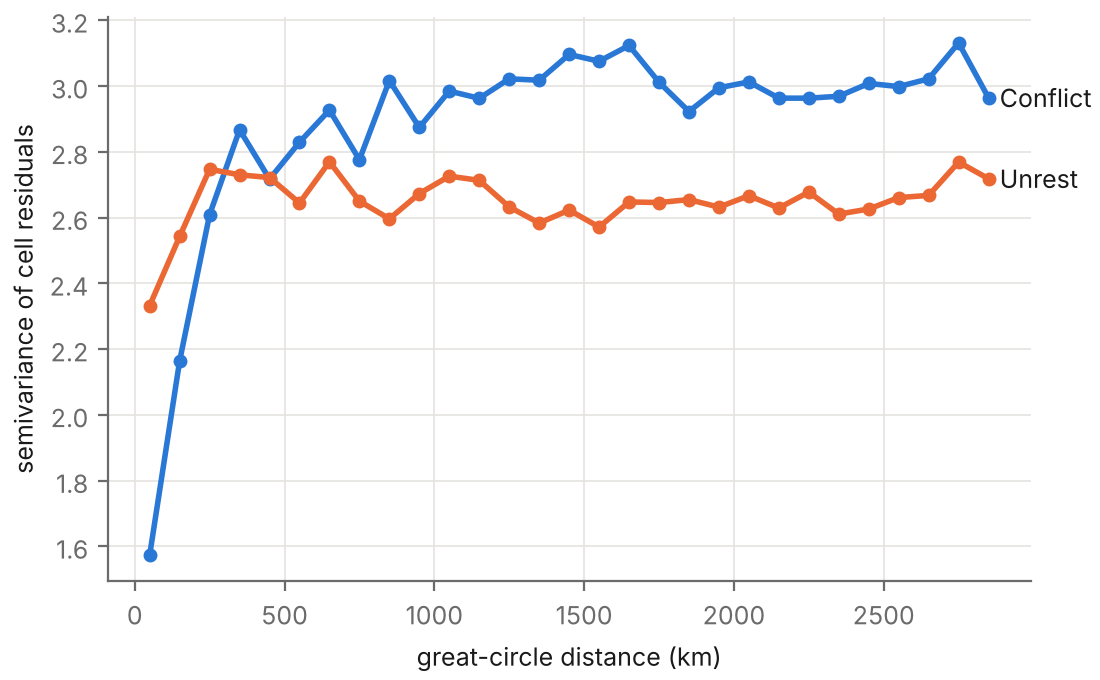
\includegraphics[width=0.6\textwidth]{figures/real_variogram.png}
\caption{Empirical semivariograms of the standardised cell residuals of the spatially
cross-fitted XGBoost model, against great-circle distance.}\label{fig:app-variogram}
\end{figure}

\subsection{State dependence, climate and national indicators}\label{sec:app-glmm}

\todo{Results of the parametric models (CRC Task 8):
(i) the state-dependence coefficient $\delta$ with lags only, with $u + w$, and with the
space-time field $v$ (Sahel and Horn of Africa);
(ii) biome means and within-biome variation of the temperature effect from the SVC model;
(iii) national indicators (EPI, footprints, GHG, V-Dem) without latent effects, with
$u + w$, and with spatial+, interpreted in the light of the confounding results of
Section~\ref{sec:sim-confounding}.}
